\chapter{Parabolic equations}
We will look at the \addtoindex{Heat equation} as our sample parabolic equation.
\[ \frac{\partial U}{\partial T}=K\frac{\partial^2U }{\partial X^2} \mbox{ on } \Omega \]
and 
\[ U=g(x,y) \mbox{ on the boundary } \delta\Omega \]
this can be transformed without loss of generality by a non-dimensional transformation to

\begin{equation}\label{heat} \frac{\partial U}{\partial t}=\frac{\partial^2U }{\partial x^2}\end{equation}

\section{An explicit method for the heat eqn}
The explicit Forwards Time Centered Space (FTCS) equation difference equation of the differential equation (\ref{heat}) is
\begin{equation}
\frac{w_{ij+1}-w_{ij}}{t_{j+1}-t_{j}}=\frac{w_{i+1j}-2w_{ij}+w_{i-1j}}{h^2},
\end{equation}

\begin{equation*}
\frac{w_{ij+1}-w_{ij}}{k}=\frac{w_{i+1j}-2w_{ij}+w_{i-1j}}{h^2}
\end{equation*}
when approaching this we have divided up the area into
two uniform meshes one in the x direction and the other in the t-direction.
We define $t_j=jk$ where k is the step size in the time direction.\\
We define $x_i=ih$ where h is the step size in the space direction.\\
$w_{ij}$ denotes the numerical approximation of $U$ at $(x_i,t_j)$.\\
Rearranging the equation we get
\begin{equation}\label{disc heat}
w_{ij+1}=rw_{i-1j}+(1-2r)w_{ij}+rw_{i+1j}
\end{equation}
where $r=\frac{k}{h^2}$.\\
This gives the formula for the unknown term $w_{ij+1}$ at the $(ij+1)$ mesh points
in terms of terms along the jth time row.\\
Hence we can calculate the unknown pivotal values of $w$ along the first row $t=k$ or $j=1$ in terms of the known boundary conditions.\\
This can be written in matrix from 
\[ \mathbf{w}_{j+1}=A\mathbf{w}_{j} +\mathbf{b}_{j} \]
for which $A$ is
\[
\left(\begin{array}{ccccccc}
1-2r&r&0&.&.&.&.\\
r&1-2r&r&0&.&.&.\\
0&r&1-2r&r&0&.&.\\
.&.&.&.&.&.&.\\
.&.&.&.&r&1-2r&r\\
.&.&.&.&.&r&1-2r\\
\end{array}\right)
\]
where $r=\frac{k}{h_x^2}>0$, $\mathbf{w}_j$ is 
\[
\left(\begin{array}{c}
w_{1j}\\
w_{2j}\\
.\\
w_{N-2j}\\
w_{N-1j}\\

\end{array}\right)
\]
and $\mathbf{b}_j$ is 
\[
\left(\begin{array}{c}
rw_{0j}\\
0\\
.\\
0\\
rw_{Nj}\\
\end{array}\right).
\]
It is assumed that the boundary values $w_{0j}$ and $w_{Nj}$ are known for $j=1,2,...$, and $w_{i0}$ is the initial condition.

\subsection{Example explicit method for the Heat Equation} 
In this case we look at a rod of unit length with each end in ice.\\
The rod is heat insulated along its length so that temperature changes occur through
heat conduction along its length and heat transfer at its ends, where w denotes
temperature.\\

\textbf{Simple case}\\
Given that the ends of the rod are kept in contact with ice and the initial temperature
distribution is non dimensional form is
\begin{enumerate}
\item $U=2x$ for $0\leq x \leq \frac{1}{2}$, 
\item $U=2(1-x)$ for $\frac{1}{2}\leq x \leq 1$. 
\end{enumerate}
In other words we are seeking a numerical solution of
\[\frac{\partial U}{\partial t}=\frac{\partial^2U }{\partial x^2}\]
which satisfies
\begin{enumerate}
\item $U=0$ at $x=0$ for all $t>0$ (the boundary condition)
\item $U=2x$ for $0\leq x \leq \frac{1}{2}$ for t=0
$U=2(1-x)$ for $\frac{1}{2}\leq x \leq 1$ for t=0 (the initial condition)
\end{enumerate}
The problem is symmetric with respect to $x=0.5$ so we need the solution only for $0\leq x \leq \frac{1}{2}$
\begin{example}
\subsubsection{Explicit FTCS method for the Heat Equation with $r=\frac{1}{10}$}
Let $h=\frac{1}{5}$ and $k=\frac{1}{250}$ so that $r=\frac{k}{h^2}=\frac{1}{10}$
difference equation (\ref{disc heat}) becomes
\[
w_{ij+1}=\frac{1}{10}(w_{i-1j}+8w_{ij}+w_{i+1j}).
\]
This can be written in matrix form 
\[
\left(\begin{array}{c}
w_{1j+1}\\
w_{2j+1}\\
w_{3j+1}\\
w_{4j+1}
\end{array}\right)
=
\left(\begin{array}{cccc}
0.8&0.1&0&0\\
0.1&0.8&0.1&0\\
0&0.1&0.8&0.1\\
0&0&0.1&0.8
\end{array}\right)
\left(\begin{array}{c}
w_{1j}\\
w_{2j}\\
w_{3j}\\
w_{4j}
\end{array}\right)+0.1\left(\begin{array}{c}
w_{0j}\\
0\\
0\\
w_{5j}
\end{array}\right).
\]
Figure \ref{Matrix_FTCS_1_10} shows a graphical representation of the matrix.
\begin{figure}[H]
  \caption{Graphical representation of the matrix A for $r=\frac{1}{10}$. }
  \centering
    \includegraphics[width=0.5\textwidth]{HeatEquationFigures/r_equals_one_tenth/Matrix}
    \label{Matrix_FTCS_1_10}
\end{figure}
To solve for $w_{21}$ we have
\[w_{21}=\frac{1}{10}(w_{10}+8w_{20}+w_{30})=\frac{1}{10}(0.4+8\times 0.8+0.8)=0.76. \]
Table \ref{Table_FTCS_1_10} shows the initial condition and one time step for the Heat Equation.
\begin{center}
 \begin{table}[H]
 \caption{The explicit numerical solution $w$ of the Heat Equation for $r=\frac{1}{10}$ for $1$ time step.}
 \label{Table_FTCS_1_10}
 \centering
\begin{tabular}{l|cccccc}
j/x&0&0.2&0.4&0.6&0.8&1.0\\ \hline
0&0&0.4&0.8&0.8&0.4&0.0\\
$\frac{1}{250}$&0&0.4&0.76&0.76&0.4&0.0
\end{tabular}
\end{table}
\end{center}

Figure \ref{Plot_FTCS_1_10} shows the explicit numerical solution $w$ of the Heat Equation for $r=\frac{1}{10}$ for $10$ time steps each represented by a different line. 
\begin{figure}[H]
  \caption{The explicit numerical solution $w$ of the Heat Equation for $r=\frac{1}{10}$ for $10$ time steps each represented by a different line.}
  \centering
    \includegraphics[width=0.5\textwidth]{HeatEquationFigures/r_equals_one_tenth/solution_plot_lines}
        \label{Plot_FTCS_1_10}

\end{figure}
Figure \ref{Color_FTCS_1_10} shows the explicit numerical solution $w$ of the Heat Equation for $r=\frac{1}{10}$ for $10$ time steps as a colour plot. 

\begin{figure}[H]
  \caption{The colour plot of the explicit numerical solution $w$ of the Heat Equation for $r=\frac{1}{10}$.}
  \centering
    \includegraphics[width=0.5\textwidth]{HeatEquationFigures/r_equals_one_tenth/solution_plot_image}
    \label{Color_FTCS_1_10}
\end{figure}
The forward time and centered space numerical solution for the Heat Equation shown in Figures \ref{Color_FTCS_1_10} and  \ref{Plot_FTCS_1_10} tends to $0$ in a monotonic fashion as time progresses for $r=\frac{1}{10}$. 
\end{example}
\begin{example}
\subsubsection{Explicit FTCS method for the Heat Equation with $r=\frac{1}{2}$}
Let $h=\frac{1}{5}$ and $k=\frac{1}{50}$ so that $r=\frac{k}{h^2}=\frac{1}{2}$
difference equation (\ref{disc heat}) becomes
\[
w_{ij+1}=\frac{1}{2}(w_{i-1j}+w_{i+1j}).
\]
This can be written in matrix form 
\[
\left(\begin{array}{c}
w_{1j+1}\\
w_{2j+1}\\
w_{3j+1}\\
w_{4j+1}
\end{array}\right)
=
\left(\begin{array}{cccc}
0.0&0.5&0&0\\
0.5&0.0&0.5&0\\
0&0.5&0.0&0.5\\
0&0&0.5&0.0
\end{array}\right)
\left(\begin{array}{c}
w_{1j}\\
w_{2j}\\
w_{3j}\\
w_{4j}
\end{array}\right)
+0.5\left(\begin{array}{c}
w_{0j}\\
0\\
0\\
w_{Nj}
\end{array}\right).
\]
Figure \ref{Matrix_FTCS_1_2} is a graphical representation of the matrix A. 
\begin{figure}[H]
  \caption{Graphical representation of the matrix A for $r=\frac{1}{2}$. }
  \centering
    \includegraphics[width=0.5\textwidth]{HeatEquationFigures/r_equals_half/Matrix}
    \label{Matrix_FTCS_1_2}
\end{figure}

Table \ref{Matrix_FTCS_1_2} shows the explicit numerical solution $w$ of the Heat Equation for $r=\frac{1}{2}$ for $1$ time step.


\begin{center}
\begin{table}[H]
 \caption{The explicit numerical solution $w$ of the Heat Equation for $r=\frac{1}{2}$ for $1$ time step.}
     \label{Table_FTCS_1_2}
 \centering
\begin{tabular}{l|cccccc}
t/x&0&0.2&0.4&0.6&0.8&1.0\\ \hline
0&0&0.4&0.8&0.8&0.4&0.0\\
$\frac{1}{50}$&0&0.4&0.6&0.6&0.4&0.0\\
\end{tabular}
\end{table}
\end{center}

Figure \ref{Plot_FTCS_1_2} shows the explicit numerical solution $w$ of the Heat Equation for $r=\frac{1}{2}$ for $10$ time steps each represented by a different line.
\begin{figure}[H]
  \caption{The explicit numerical solution $w$ of the Heat Equation for $r=\frac{1}{2}$ for $10$ time steps each represented by a different line.}
  \centering
    \includegraphics[width=0.5\textwidth]{HeatEquationFigures/r_equals_half/solution_plot_lines}     \label{Plot_FTCS_1_2}

\end{figure}
Figure \ref{Color_FTCS_1_2} shows the explicit numerical solution $w$ of the Heat Equation for $r=\frac{1}{2}$ for $10$ time steps as a colour plot.

\begin{figure}[H]
  \caption{The colour plot of the explicit numerical solution $w$ of the Heat Equation for $r=\frac{1}{2}$.}
  \centering
    \includegraphics[width=0.5\textwidth]{HeatEquationFigures/r_equals_half/solution_plot_image}\label{Color_FTCS_1_2}
\end{figure}


The choice of $r=\frac{1}{2}$  gives an acceptable approximation to the solution of the \addtoindex{Heat Equation} as shown in Figures  \ref{Plot_FTCS_1_2} and \ref{Color_FTCS_1_2}.
\end{example}
\begin{example}
\subsubsection{Explicit FTCS method for the Heat Equation with $r=1$}
Let $h=\frac{1}{5}$ and $k=\frac{1}{25}$ so that $r=\frac{k}{h^2}=1$
difference equation (\ref{disc heat}) becomes
\[
w_{ij+1}=w_{i-1j}-w_{ij}+w_{i+1j}.
\]
This can be written in matrix form 
\[
\left(\begin{array}{c}
w_{1j+1}\\
w_{2j+1}\\
w_{3j+1}\\
w_{4j+1}
\end{array}\right)
=
\left(\begin{array}{cccc}
-1.0&1.0&0&0\\
1.0&-1.0&1.0&0\\
0&1.0&-1.0&1.0\\
0&0&1.0&-1.0
\end{array}\right)
\left(\begin{array}{c}
w_{1j}\\
w_{2j}\\
w_{3j}\\
w_{4j}
\end{array}\right)\]\[+\left(\begin{array}{c}
w_{0j}\\
0\\
0\\
w_{5j}
\end{array}\right).
\]
\begin{figure}[H]
  \caption{Graphical representation of the matrix A for $r=1$.}
  \centering
    \includegraphics[width=0.5\textwidth]{HeatEquationFigures/r_equals_one/Matrix}
\end{figure}


\begin{center}
\begin{table}[H]
 \caption{The explicit numerical solution $w$ of the Heat Equation for $r=1$ for 3 time steps.}
 \centering
\begin{tabular}{l|cccccc}
t/x&0&0.2&0.4&0.6&0.8&1.0\\ \hline
0&0&0.4&0.8&0.8&0.4&0.0\\
$\frac{1}{25}$&0&0.4&0.4&0.4&0.4&0.0\\
$\frac{2}{25}$&0&0.0&0.4&0.4&0.0&0.0\\
$\frac{3}{25}$&0&0.4&0.0&0.0&0.4&0.0\\
\end{tabular}
\end{table}
\end{center}

\begin{figure}[H]
  \caption{The explicit numerical solution $w$ of the Heat Equation for $r=1$ for 10 time steps each represented by a different line.}
  \centering
    \includegraphics[width=0.5\textwidth]{HeatEquationFigures/r_equals_one/solution_plot_lines}
\end{figure}


\begin{figure}[H]
  \caption{The colorplot of The explicit numerical solution $w$ of the Heat Equation for $r=1$.}
  \centering
    \includegraphics[width=0.5\textwidth]{HeatEquationFigures/r_equals_one/solution_plot_image}
\end{figure}

Considered as a solution to the \addtoindex{Heat Equation} this is meaningless although it is the correct
solution of the difference equation with respect to the initial conditions and the boundary conditions.
\end{example}
\section{An implicit (BTCS) method for the Heat Equation}
The  implicit Backward Time Centered Space (BTCS) difference equation of the differential Heat equation (\ref{heat}) is
\begin{equation}
\frac{w_{ij+1}-w_{ij}}{k}=\frac{w_{i+1j+1}-2w_{ij+1}+w_{i-1j+1}}{h^2}
\end{equation}
when approaching this we have divided up the area into
two uniform meshes one in the $x$ direction and the other in the $t$-direction.
We define $t_j=jk$ where $k$ is the step size in the time direction.\\
We define $x_i=ih$ where $h$ is the step size in the space direction.\\
$w_{ij}$ denotes the numerical approximation of $U$ at $(x_i,t_j)$.\\
Rearranging the equation we get
\begin{equation}\label{disc heat imp}
-rw_{i-1j+1}+(1+2r)w_{ij+1}-rw_{i+1j+1}=w_{ij}
\end{equation}
where $r=\frac{k}{h^2}$.\\
This gives the formula for the unknown term $w_{ij+1}$ at the $(ij+1)$ mesh points
in terms of terms along the jth time row.\\
Hence we can calculate the unknown pivotal values of $w$ along the first row $t=k$ or $j=1$ in terms of the known boundary conditions.\\
This can be written in matrix from 
\[ A\mathbf{w}_{j+1}=\mathbf{w}_{j} +\mathbf{b}_{j+1} \]
for which $A$ is
\[
\left(\begin{array}{ccccccc}
1+2r&-r&0&.&.&.&.\\
-r&1+2r&-r&0&.&.&.\\
0&-r&1+2r&-r&0&.&.\\
.&.&.&.&.&.&.\\
.&.&.&.&-r&1+2r&-r\\
.&.&.&.&.&-r&1+2r\\
\end{array}\right)
\]
where $r=\frac{k}{h_x^2}>0$, $\mathbf{w}_j$ is 
\[
\left(\begin{array}{c}
w_{1j}\\
w_{2j}\\
.\\
w_{N-2j}\\
w_{N-1j}\\

\end{array}\right)
\]
and $\mathbf{b}_{j+1}$ is 
\[
\left(\begin{array}{c}
rw_{0j+1}\\
0\\
.\\
0\\
rw_{Nj+1}\\
\end{array}\right).
\]
It is assumed that the boundary values $w_{0j}$ and $w_{Nj}$ are known for $j=1,2,...$, and $w_{i0}$ is the initial condition.

\subsection{Example implicit (BTCS) for the Heat Equation} 
In this case we look at a rod of unit length with each end in ice.\\
The rod is heat insulated along its length so that temperature changes occur through
heat conduction along its length and heat transfer at its ends, where $w$ denotes
temperature.\\
Given that the ends of the rod are kept in contact with ice and the initial temperature
distribution is non dimensional form is
\begin{enumerate}
\item $U=2x$ for $0\leq x \leq \frac{1}{2}$ 
\item $U=2(1-x)$ for $\frac{1}{2}\leq x \leq 1$ 
\end{enumerate}
In other words we are seeking a numerical solution of
\[\frac{\partial U}{\partial t}=\frac{\partial^2U }{\partial x^2}\]
which satisfies
\begin{enumerate}
\item $U=0$ at $x=0$ for all $t>0$ (the boundary condition),
\item $U=2x$ for $0\leq x \leq \frac{1}{2}$ for $t=0$,\\
$U=2(1-x)$ for $\frac{1}{2}\leq x \leq 1$ for $t=0$ (the initial condition).
\end{enumerate}
\begin{example}
\subsubsection{Implicit (BTCS) method for the Heat Equation  $r=\frac{1}{10}$}
Let $h=\frac{1}{5}$ and $k=\frac{1}{250}$ so that $r=\frac{k}{h^2}=\frac{1}{10}$
difference equation (\ref{disc heat}) becomes
\[
\frac{1}{10}(-w_{i-1j+1}+(12)w_{ij+1}-w_{i+1j+1})=w_{ij}
\]
This can be written in matrix form 
\[
\left(\begin{array}{cccc}
1.2&-0.1&0&0\\
-0.1&1.2&-0.1&0\\
0&-0.1&1.2&-0.1\\
0&0&-0.1&1.2
\end{array}\right)
\left(\begin{array}{c}
w_{1j+1}\\
w_{2j+1}\\
w_{3j+1}\\
w_{4j+1}
\end{array}\right)
=
\left(\begin{array}{c}
w_{1j}\\
w_{2j}\\
w_{3j}\\
w_{4j}
\end{array}\right)+0.1\left(\begin{array}{c}
w_{0j+1}\\
0\\
0\\
w_{5j+1}
\end{array}\right).
\]
\begin{figure}[H]
  \caption{Graphical representation of the matrix A for $r=\frac{1}{10}$. }
  \centering
    \includegraphics[width=0.5\textwidth]{HeatEquationFigures/Fully_implicit/r_equals_one_tenth/Matrix}
\end{figure}


To solve we need to invert the matix, to get
\[ \mathbf{w}_{j+1}=A^{-1}(\mathbf{w}_{j} +\mathbf{b}_{j}) \]


\begin{center}
 \begin{table}[H]
 \caption{The implicit numerical solution $w$ of the Heat Equation for $r=\frac{1}{10}$ for 1 time step.}
 \centering
\begin{tabular}{l|cccccc}
j/x&0&0.2&0.4&0.6&0.8&1.0\\ \hline
0&0&0.4&0.8&0.8&0.4&0.0\\
$\frac{1}{250}$&
 0.&          0.39694656 & 0.76335878 & 0.76335878 & 0.39694656&  0.
\end{tabular}
\end{table}
\end{center}

\begin{figure}[H]
  \caption{The implicit numerical solution $w$ of the Heat Equation for $r=\frac{1}{10}$ for $10$ time steps each represented by a different line.}
  \centering
    \includegraphics[width=0.5\textwidth]{HeatEquationFigures/Fully_implicit/r_equals_one_tenth/solution_plot_lines}
\end{figure}


\begin{figure}[H]
  \caption{The colorplot of The implicit numerical solution $w$ of the Heat Equation for $r=\frac{1}{10}$.}
  \centering
    \includegraphics[width=0.5\textwidth]{HeatEquationFigures/Fully_implicit/r_equals_one_tenth/solution_plot_image}
\end{figure}
\end{example}

\begin{example}


\subsubsection{Implicit (BTCS) method for the Heat Equation for $r=\frac{1}{2}$}
Let $h=\frac{1}{5}$ and $k=\frac{1}{50}$ so that $r=\frac{k}{h^2}=\frac{1}{2}$
difference equation (\ref{disc heat}) becomes
\[
\frac{1}{2}(-w_{i-1j+1}+(4)w_{ij+1}-w_{i+1j+1})=w_{ij}
\]
This can be written in matrix form 
\[
\left(\begin{array}{cccc}
2&-0.5&0&0\\
-0.5&2&-0.5&0\\
0&-0.5&2&-0.5\\
0&0&-0.5&2
\end{array}\right)
\left(\begin{array}{c}
w_{1j+1}\\
w_{2j+1}\\
w_{3j+1}\\
w_{4j+1}
\end{array}\right)
=
\left(\begin{array}{c}
w_{1j}\\
w_{2j}\\
w_{3j}\\
w_{4j}
\end{array}\right).
\]
\begin{figure}[H]
  \caption{Graphical representation of the matrix A for $r=\frac{1}{2}$ }
  \centering
    \includegraphics[width=0.5\textwidth]{HeatEquationFigures/Fully_implicit/r_equals_half/Matrix}
\end{figure}


\begin{center}
\begin{table}[H]
 \caption{The implicit numerical solution $w$ of the Heat Equation for $r=\frac{1}{2}$ for $1$ time step}
 \centering
\begin{tabular}{l|cccccc}
t/x&0&0.2&0.4&0.6&0.8&1.0\\ \hline
0&0&0.4&0.8&0.8&0.4&0.0\\
$\frac{1}{50}$&0. &         0.36363636 &  0.65454545 & 0.65454545&  0.36363636 & 0.
\end{tabular}
\end{table}
\end{center}

\begin{figure}[H]
  \caption{The implicit numerical solution $w$ of the Heat Equation for $r=\frac{1}{2}$ for $10$ time steps each represented by a different line}
  \centering
    \includegraphics[width=0.5\textwidth]{HeatEquationFigures/Fully_implicit/r_equals_half/solution_plot_lines}
\end{figure}


\begin{figure}[H]
  \caption{The colorplot of the implicit numerical solution $w$ of the Heat Equation for $r=\frac{1}{2}$.}
  \centering
    \includegraphics[width=0.5\textwidth]{HeatEquationFigures/Fully_implicit/r_equals_half/solution_plot_image}
\end{figure}


This method also gives an acceptable approximation to the solution of the \addtoindex{PDE}.
\end{example}
\begin{example}
\subsubsection{Implicit (BTCS) method for the Heat Equation for $r=1$}
Let $h=\frac{1}{5}$ and $k=\frac{1}{25}$ so that $r=\frac{k}{h^2}=1$
difference equation (\ref{disc heat}) becomes
\[
(-w_{i-1j+1}+(3)w_{ij+1}-w_{i+1j+1})=w_{ij}
\]
This can be written in matrix form 
\[
\left(\begin{array}{cccc}
3&-1&0&0\\
-1&3&-1&0\\
0&-1&3&-1\\
0&0&-1&3
\end{array}\right)
\left(\begin{array}{c}
w_{1j+1}\\
w_{2j+1}\\
w_{3j+1}\\
w_{4j+1}
\end{array}\right)
=
\left(\begin{array}{c}
w_{1j}\\
w_{2j}\\
w_{3j}\\
w_{4j}
\end{array}\right)+\left(\begin{array}{c}
w_{0j+1}\\
0\\
0\\
w_{5j+1}
\end{array}\right).
\]
\begin{figure}[H]
  \caption{Graphical representation of the matrix A for $r=1$ }
  \centering
    \includegraphics[width=0.5\textwidth]{HeatEquationFigures/Fully_implicit/r_equals_one/Matrix}
\end{figure}


\begin{center}
\begin{table}[H]
 \caption{The implicit numerical solution $w$ of the Heat Equation for $r=1$ for 3 time step}
 \centering
\begin{tabular}{l|cccccc}
t/x&0&0.2&0.4&0.6&0.8&1.0\\ \hline
0&0&0.4&0.8&0.8&0.4&0.0\\
$\frac{1}{25}$&0.  &  0.32  &0.56&  0.56 & 0.32  &0.\\
$\frac{2}{25}$&0. &   0.24 & 0.4  & 0.4  & 0.24 & 0.\\
$\frac{3}{25}$&0. &    0.176&  0.288 & 0.288 & 0.176 & 0. 
\end{tabular}
\end{table}
\end{center}

\begin{figure}[H]
  \caption{The implicit numerical solution $w$ of the Heat Equation for $r=1$ for 10 time steps each represented by a different line}
  \centering
    \includegraphics[width=0.5\textwidth]{HeatEquationFigures/Fully_implicit/r_equals_one/solution_plot_lines}
\end{figure}


\begin{figure}[H]
  \caption{The colorplot of the implicit numerical solution $w$ of the Heat Equation for $r=1$.}
  \centering
    \includegraphics[width=0.5\textwidth]{HeatEquationFigures/Fully_implicit/r_equals_one/solution_plot_image}
\end{figure}
\end{example}


\section{Crank Nicholson Implicit method}
Since the implicit method requires that $k\leq \frac{1}{2}h^2$ a new method was
needed which would work for all finite values of r.\\
They considered the partial differential equation as being satisfied at the
midpoint $\{ih,(j+\frac{1}{2})k \}$ and replace $\frac{\delta^2 U}{\delta x^2}$ by the
mean of its finite difference approximations at the jth and (j+1)th time levels.
In other words they approximated the equation
\[ \left(\frac{\delta U}{\delta t}\right)_{i,j+\frac{1}{2}}
= 
 \left(\frac{\delta^2 U}{\delta x^2}\right)_{i,j+\frac{1}{2}}\]
by
\[\frac{w_{i,j+1}-w_{ij}}{k}=\frac{1}{2}\left\{\frac{w_{i+1j+1}-2w_{ij+1}+w_{i-1j+1}}{h^2}+
\frac{w_{i+1j}-2w_{ij}+w_{i-1j}}{h^2}
\right\}
\]
giving
\begin{equation}
\label{2 crank}
-rw_{i-1j+1}+(2+2r)w_{ij+1}-rw_{i+1j+1}
=
rw_{i-1j}+(2-2r)w_{ij}+rw_{i+1j}
\end{equation}

with $r=\frac{k}{h^2}$.\\
In general the LHS contains $3$ unknowns and the RHS $3$ known pivotal values.\\
If there are N intervals mesh points along each row then for $j=0$ and $i=1,..,N$ it 
gives N simultaneous equations for $N$ unknown pivotal values along the first row.\\
Which can be described in matrix form 
\[ B \mathbf{w}_{j+1}=C\mathbf{w}_{j}+\mathbf{b}_{j}\]
as
\begin{eqnarray*}
\left(\begin{array}{ccccccc}
2+2r&-r&0&.&.&.&.\\
-r&2+2r&-r&0&.&.&.\\
0&-r&2+2r&-r&0&.&.\\
.&.&.&.&.&.&.\\
.&.&.&.&-r&2+2r&-r\\
.&.&.&.&.&-r&2+2r\\
\end{array}\right)
\left(\begin{array}{c}
w_{1j+1}\\
w_{2j+1}\\
.\\
.\\
w_{N-2j+1}\\
w_{N-1j+1}\\
\end{array}\right)\\
=
\left(\begin{array}{ccccccc}
2-2r&r&0&.&.&.&.\\
r&2-2r&r&0&.&.&.\\
0&r&2-2r&r&0&.&.\\
.&.&.&.&.&.&.\\
.&.&.&.&r&2-2r&r\\
.&.&.&.&.&r&2-2r\\
\end{array}\right)
\left(\begin{array}{c}
w_{1j}\\
w_{2j}\\
.\\
.\\
w_{N-2j}\\
w_{N-1j}\\
\end{array}\right)
+\mathbf{b}_j+\mathbf{b}_{j+1}
\end{eqnarray*}
where $\mathbf{b}_j$ and $\mathbf{b}_{j+1}$ are vectors of known boundary conditions. 
\begin{equation}
    \mathbf{b}_j=\left(\begin{array}{c}
rw_{0j}\\
0\\
.\\
.\\
0\\
rw_{Nj}\\
\end{array}\right), \ \ \     
\mathbf{b}_{j+1}=\left(\begin{array}{c}
rw_{0j+1}\\
0\\
.\\
.\\
0\\
rw_{Nj+1}\\
\end{array}\right)
\end{equation}

\subsection{Example Crank-Nicholson solution of the Heat Equation} 
In this case we look at a rod of unit length with each end in ice.\\
The rod is heat insulated along its length so that temperature changes occur through
heat conduction along its length and heat transfer at its ends, where w denotes
temperature.\\
\textbf{Simple case}\\
Given that the ends of the rod are kept in contact with ice and the initial temperature
distribution is non dimensional form is
\begin{enumerate}
\item $U=2x$ for $0\leq x \leq \frac{1}{2}$ 
\item $U=2(1-x)$ for $\frac{1}{2}\leq x \leq 1$ 
\end{enumerate}
In other words we are seeking a numerical solution of
\[\frac{\partial U}{\partial t}=\frac{\partial^2U }{\partial x^2}\]
which satisfies
\begin{enumerate}
\item $U=0$ at $x=0$ for all $t>0$ (the boundary condition)
\item $U=2x$ for $0\leq x \leq \frac{1}{2}$ for $t=0$
$U=2(1-x)$ for $\frac{1}{2}\leq x \leq 1$ for $t=0$ (the initial condition)
\end{enumerate}
\begin{example}
\subsubsection{Crank-Nicholson method $r=\frac{1}{10}$}
Let $h=\frac{1}{5}$ and $k=\frac{1}{250}$ so that $r=\frac{k}{h^2}=\frac{1}{10}$
difference equation (\ref{2 crank}) becomes
\[-0.1w_{i-1,j+1}+2.2w_{i,j+1}-0.1w_{i+1,j+1}=0.1w_{i-1,j}+1.8w_{i,j}+0.1w_{i+1,j} \]
Let $j=0$
\[\begin{array}{lcl}
i=1:& &\\
-0.1w_{0,1}+2.2w_{1,1}-0.1w_{2,1}&=&0.1w_{0,0}+1.8w_{1,0}+0.1w_{2,0}\\
i=2:& &\\
-0.1w_{1,1}+2.2w_{2,1}-0.1w_{3,1}&=&0.1w_{1,0}+1.8w_{2,0j}+0.1w_{3,0}\\
i=3:& &\\
-0.1w_{2,1}+2.2w_{3,1}-0.1w_{4,1}&=&0.1w_{2,0}+1.8w_{3,0}+0.1w_{4,0}\\
i=4:& &\\
-0.1w_{3,1}+2.2w_{4,1}-0.1w_{5,1}&=&0.1w_{3,0}+1.8w_{4,0}+0.1w_{5,0}
\end{array}\]
In matrix form
\[\left(\begin{array}{cccc}
2.2&-0.1&0&0\\
-0.1&2.2&-0.1&0\\
0&-0.1&2.2&-0.1\\
0&0&-0.1&2.2
\end{array}
\right)
\left(\begin{array}{c}
w_{1,1}\\
w_{2,1}\\
w_{3,1}\\
w_{4,1}\\
\end{array}
\right)\]\[=\left(\begin{array}{cccc}
1.8&0.1&0&0\\
0.1&1.8&0.1&0\\
0&0.1&1.8&0.1\\
0&0&0.1&1.8\\

\end{array}
\right)
\left(\begin{array}{c}
w_{1,0}\\
w_{2,0}\\
w_{3,0}\\
w_{4,0}
\end{array}
\right)+0.1
\left(\begin{array}{c}
w_{0,1}+w_{0,0}\\
0\\
0\\
w_{5,1}+w_{5,0}\\
\end{array}
\right)
\]	

To solve we need to invert the matix, to get
\[ \mathbf{w}_{j+1}=A^{-1}(B\mathbf{w}_{j} +\mathbf{b}_{j+1}+\mathbf{b}_{j}) \]


\begin{center}
 \begin{table}[H]
 \caption{The Crank-Nicholson numerical solution $w$ of the Heat Equation for $r=\frac{1}{10}$ for 1 time step}
 \centering
\begin{tabular}{l|cccccc}
j/x&0&0.2&0.4&0.6&0.8&1.0\\ \hline
0&0&0.4&0.8&0.8&0.4&0.0\\
$\frac{1}{250}$&
 0.   &       0.39826464  &0.76182213 & 0.76182213 & 0.39826464&  0.
\end{tabular}
\end{table}
\end{center}

\begin{figure}[H]
  \caption{The Crank-Nicholson numerical solution $w$ of the Heat Equation for $r=\frac{1}{10}$ for 10 time steps each represented by a different line}
  \centering
    \includegraphics[width=0.5\textwidth]{HeatEquationFigures/CRN/r_equals_one_tenth/solution_plot_lines}
\end{figure}


\begin{figure}[H]
  \caption{The colorplot of the Crank-Nicholson numerical solution $w$ of the Heat Equation for $r=\frac{1}{10}$.}
  \centering
    \includegraphics[width=0.5\textwidth]{HeatEquationFigures/CRN/r_equals_one_tenth/solution_plot_image}
\end{figure}

\end{example}
\begin{example}
\subsubsection{Crank-Nicholson method $r=\frac{1}{2}$}
Let $h=\frac{1}{5}$ and $k=\frac{1}{50}$ so that $r=\frac{k}{h^2}=\frac{1}{2}$
difference equation (\ref{2 crank}) becomes
\[-0.5w_{i-1,j+1}+3w_{i,j+1}-0.5w_{i+1,j+1}=\]
\[
0.5w_{i-1,j}+1w_{i,j}+0.5w_{i+1,j} \]
Let $j=0$
\[\begin{array}{lcl}
i=1:&\\
-0.5w_{0,1}+3w_{1,1}-0.5w_{2,1}&=&0.5w_{0,0}+1w_{1,0}+0.5w_{2,0}\\
i=2:&\\
-0.5w_{1,1}+3w_{2,1}-0.5w_{3,1}&=&0.5w_{1,0}+1w_{2,0j}+0.5w_{3,0}\\
i=3:&\\
-0.5w_{2,1}+3w_{3,1}-0.5w_{4,1}&=&0.5w_{2,0}+1w_{3,0}+0.5w_{4,0}\\
i=4:&\\
-0.5w_{3,1}+3w_{4,1}-0.5w_{5,1}&=&0.5w_{3,0}+1w_{4,0}+0.5w_{5,0}
\end{array}\]
In matrix form
\[\left(\begin{array}{cccc}
3&-0.5&0&0\\
-0.5&3&-0.5&0\\
0&-0.5&3&-0.5\\
0&0&-0.5&3
\end{array}
\right)
\left(\begin{array}{c}
w_{1,1}\\
w_{2,1}\\
w_{3,1}\\
w_{4,1}\\
\end{array}
\right)=\]\
\[\left(\begin{array}{cccc}
1&0.5&0&0\\
0.5&1&0.5&0\\
0&0.5&1&0.5\\
0&0&0.5&1\\

\end{array}
\right)
\left(\begin{array}{c}
w_{1,0}\\
w_{2,0}\\
w_{3,0}\\
w_{4,0}
\end{array}
\right)+0.5
\left(\begin{array}{c}
w_{0,1}+w_{0,0}\\
0\\
0\\
w_{5,1}+w_{5,0}\\
\end{array}
\right)
\]	



\begin{center}
\begin{table}[H]
 \caption{The Crank-Nicholson numerical solution $w$ of the Heat Equation for $r=\frac{1}{2}$ for 1 time step}
 \centering
\begin{tabular}{l|cccccc}
t/x&0&0.2&0.4&0.6&0.8&1.0\\ \hline
0&0&0.4&0.8&0.8&0.4&0.0\\
$\frac{1}{50}$&0.    &      0.37241379  & 0.63448276 & 0.63448276  & 0.37241379 & 0.
\end{tabular}
\end{table}
\end{center}

\begin{figure}[H]
  \caption{The Crank-Nicholson numerical solution $w$ of the Heat Equation for $r=\frac{1}{2}$ for 10 time steps each represented by a different line}
  \centering
    \includegraphics[width=0.5\textwidth]{HeatEquationFigures/CRN/r_equals_half/solution_plot_lines}
\end{figure}


\begin{figure}[H]
  \caption{The colorplot of the Crank-Nicholson numerical solution $w$ of the Heat Equation for $r=\frac{1}{2}$.}
  \centering
    \includegraphics[width=0.5\textwidth]{HeatEquationFigures/CRN/r_equals_half/solution_plot_image}
\end{figure}


This method also gives an good approximation to the solution of the \addtoindex{PDE}.
\end{example}
\begin{example}

\subsubsection{Crank-Nicholson method for the Heat Equation with  $r=1$}
Let $h=\frac{1}{5}$ and $k=\frac{1}{25}$ so that $r=\frac{k}{h^2}=1$
difference equation (\ref{2 crank}) becomes
\[-w_{i-1,j+1}+4w_{i,j+1}-w_{i+1,j+1}=w_{i-1,j}+0w_{i,j}+w_{i+1,j} \]
Let $j=0$
\[\begin{array}{lcl}
i=1:& &\\
-w_{0,1}+4w_{1,1}-w_{2,1}&=&w_{0,0}+0w_{1,0}+w_{2,0}\\
i=2:& &\\
-w_{1,1}+4w_{2,1}-w_{3,1}&=&w_{1,0}+0w_{2,0j}+w_{3,0}\\
i=3:& &\\
-w_{2,1}+4w_{3,1}-w_{4,1}&=&w_{2,0}+0w_{3,0}+w_{4,0}\\
i=4:& &\\
-w_{3,1}+4w_{4,1}-w_{5,1}&=&w_{3,0}+0w_{4,0}+w_{5,0}
\end{array}\]
In matrix form
\[\left(\begin{array}{cccc}
4&-1&0&0\\
-1&4&-1&0\\
0&-1&4&-1\\
0&0&-1&4
\end{array}
\right)
\left(\begin{array}{c}
w_{1,1}\\
w_{2,1}\\
w_{3,1}\\
w_{4,1}\\
\end{array}
\right)\]
\[=\left(\begin{array}{cccc}
0&1&0&0\\
1&0&1&0\\
0&1&0&1\\
0&0&1&0\\

\end{array}
\right)
\left(\begin{array}{c}
w_{1,0}\\
w_{2,0}\\
w_{3,0}\\
w_{4,0}
\end{array}
\right)+
\left(\begin{array}{c}
w_{0,1}+w_{0,0}\\
0\\
0\\
w_{5,1}+w_{5,0}\\
\end{array}
\right)
\]	




\begin{center}
\begin{table}[H]
 \caption{The Crank-Nicholson numerical solution $w$ of the Heat Equation for $r=1$ for 3 time step}
 \centering
\begin{tabular}{l|cccccc}
t/x&0&0.2&0.4&0.6&0.8&1.0\\ \hline
0&0&0.4&0.8&0.8&0.4&0.0\\
$\frac{1}{25}$&0.  &        0.32727273&  0.50909091 & 0.50909091&  0.32727273&  0.\\
$\frac{2}{25}$&0.      &    0.21487603 & 0.35041322 & 0.35041322&  0.21487603 & 0.\\

$\frac{3}{25}$&0.    &      0.14695718&  0.23741548  &0.23741548&  0.14695718&  0. 
\end{tabular}
\end{table}
\end{center}

\begin{figure}[H]
  \caption{The Crank-Nicholson numerical solution $w$ of the Heat Equation for $r=1$ for 10 time steps each represented by a different line}
  \centering
    \includegraphics[width=0.5\textwidth]{HeatEquationFigures/CRN/r_equals_one/solution_plot_lines}
\end{figure}


\begin{figure}[H]
  \caption{The colorplot of the Crank-Nicholson numerical solution $w$ of the Heat Equation for $r=1$.}
  \centering
    \includegraphics[width=0.5\textwidth]{HeatEquationFigures/CRN/r_equals_one/solution_plot_image}
\end{figure}

\end{example}




\section{The Theta Method}
The Theta Method is a generalization of the Crank-Nicholson method and expresses
our partial differential equation as
\begin{equation}
\label{2 theta}
\frac{w_{i,j+1}-w_{ij}}{k}=\left\{\theta\left(\frac{w_{i+1j+1}-2w_{ij+1}+w_{i-1j+1}}{h^2}\right)+
(1-\theta)\left(
\frac{w_{i+1j}-2w_{ij}+w_{i-1j}}{h^2}
\right)
\right\}
\end{equation}
\begin{itemize}
\item
when $\theta=0$ we get the explicit scheme,
\item
when $\theta=\frac{1}{2}$ we get the Crank-Nicholson scheme,
\item
and $\theta=1$ we get fully implicit backward finite difference method.
\end{itemize}
The equations are unconditionally valid for $\frac{1}{2}\leq \theta \leq 1$.
For  $0\leq \theta < \frac{1}{2}$ we must have
\[r\leq \frac{1}{2(1-2\theta)}. \]
\section{The General Matrix form}
Let the solution domain of the \addtoindex{PDE} be the finite rectangle $0\leq x \leq 1$ and
$0\leq t \leq T$ and subdivide it into a uniform rectangular mesh by the lines
$x_i=ih$ for $i=0$ to $N$ and $t_{j}=jk$ for $j=0$ to $J$ it will be assumed that $h$ is related to $k$ by some relationship such as $k=rh$ or $k=rh^2$ with $r>0$ and finite so that as $h\rightarrow 0$ as $k \rightarrow 0$.\\
Assume that the finite difference equation relating the mesh point values along the $(j+1)$th and jth row is 
\[b_{i-1}w_{i-1j+1}+
b_{i}w_{ij+1}+
b_{i+1}w_{i+1j+1}
=
c_{i-1}w_{i-1j}+
c_{i}w_{ij}+
c_{i+1}w_{i+1j}\]
where the coefficients are constant. If the boundary values at $i=0$ and $N$ for $j>0$ are known these $(N-1)$ equations for $i=1$ to $N-1$ can be written in 
matrix form.
\begin{eqnarray*}
\left(\begin{array}{ccccccc}
b_1&b_2&0&.&.&.&.\\
b_1&b_2&b_3&0&.&.&.\\
0&b_2&b_3&b_4&0&.&.\\
.&.&.&.&.&.&.\\
.&.&.&.&b_{N-3}&b_{N-2}&b_{N-1}\\
.&.&.&.&.&b_{N-2}&b_{N-1}\\
\end{array}\right)
\left(\begin{array}{c}
w_{1j+1}\\
w_{2j+1}\\
.\\
.\\
w_{N-2j+1}\\
w_{N-1j+1}\\
\end{array}\right)
\\
=
\left(\begin{array}{ccccccc}
c_1&c_2&0&.&.&.&.\\
c_1&c_2&c_3&0&.&.&.\\
0&c_2&c_3&c_4&0&.&.\\
.&.&.&.&.&.&.\\
.&.&.&.&c_{N-3}&c_{N-2}&c_{N-1}\\
.&.&.&.&.&c_{N-2}&c_{N-1}\\
\end{array}\right)
\left(\begin{array}{c}
w_{1j}\\
w_{2j}\\
.\\
.\\
w_{N-2j}\\
w_{N-1j}\\
\end{array}\right)
+
\left(\begin{array}{c}
c_0w_{0j}-b_0w_{0j+1}\\
0\\
.\\
.\\
0\\
c_Nw_{Nj}-b_{N}w_{Nj+1}\\
\end{array}\right)
\end{eqnarray*}
Which can be written as
\[ B\mathbf{w}_{j+1}=C\mathbf{w}_j+\mathbf{d}_j \]
Where B and C are of order $(N-1)$ $\mathbf{w}_j$ denotes a column vector and
$\mathbf{d}_j$ denotes a column vector of boundary values.\\
Hence
\[ \mathbf{w}_{j+1}=B^{-1}C\mathbf{w}_j+B^{-1}\mathbf{d}_j. \]
Expressed in a more conventional manner as
\[ \mathbf{w}_{j+1}=A\mathbf{w}_j+\mathbf{f}_j \]
Where $A=B^{-1}C$ and $\mathbf{f}_j =B^{-1}\mathbf{d}_j$.  

\section{Derivative Boundary Conditions}
Boundary conditions expressed in terms of derivatives occur frequently.
\subsection{Example Derivative Boundary Conditions}
\[
\frac{\partial U}{\partial x} = H(U-v_0) \ \ \ at \ x=0\]
where H is a positive constant and $v_0$ is the surrounding temperature.\\

How do we deal with this type of boundary condition?\\

\begin{enumerate}
\item
By using forward difference for $\frac{\partial U}{\partial x}$, we have
\[
\frac{w_{1j}-w_{0j}}{h_x} = H(w_{0j}-v_0)\]
where $h_x=x_1-x_0$.  This gives us one extra equation for the temp $w_{ij}$.\\
\item
If we wish to represent $\frac{\partial U}{\partial x}$ more accurately at x=0, we use a central difference formula.  It is necessary to introduce a fictitious
temperature $w_{-1j}$ at the external mesh points $(-h_x,jk)$.  The temperature $w_{-1j}$ is unknown and needs another equation.  This is obtained by assuming that the heat 
conduction equation is satisfied at the end points.  The unknown $w_{-1j}$ can be 
eliminated between these equations.\\
\end{enumerate}
%{Example}\\
Solve for the equation
\[\frac{\partial U}{\partial t} =\frac{\partial^2 U}{\partial x^2} \]
satisfying the initial condition
\[U=1 \mbox{ for } 0\leq x \leq 1 \mbox{ when } t=0 \]
and the boundary conditions
\[\frac{\partial U}{\partial x} = U \mbox{ at } x=0 \mbox{ for all t} \]
\[\frac{\partial U}{\partial x} = -U \mbox{ at } x=1 \mbox{ for all t}. \]
\subsubsection{Example 1}
Using forward difference approximation for the derivative boundary condition
and the explicit method to approximate the \addtoindex{PDE}.\\
Our difference equation is,
\[
\frac{w_{i,j+1}-w_{ij}}{k}=
\frac{w_{i+1j}-2w_{ij}+w_{i-1j}}{h^2}
\]
\begin{equation}
\label{explicit forward}
w_{ij+1}=w_{ij} +r(w_{i-1j}-2w_{ij}+w_{i+1j})
\end{equation}
where $r=\frac{k}{h^{2}_x}$.\\
At i=1, (\ref{explicit forward}) is,
\begin{equation}
\label{explicit forward i=1}
w_{1j+1}=w_{1j} +r(w_{0j}-2w_{1j}+w_{2j})
\end{equation}
The boundary condition at $x=0$ is $\frac{\partial U}{\partial x} = U$ in terms of
forward difference this is 
\[ \frac{w_{1j}-w_{0j}}{h_x} = w_{0j}\]
rearranging 
\begin{equation}
\label{forward bc}
w_{0j}=\frac{w_{1j}}{1+h_x}
\end{equation}
Using (\ref{forward bc}) and (\ref{explicit forward i=1}) to eliminate we get,
\[w_{1j+1} = \left(1-2r+\frac{r}{1+h_x}\right)w_{1j}+rw_{2j}.\]


At $i=N-1$, (\ref{explicit forward}) is,
\begin{equation}
\label{explicit forward i=N-1}
w_{N-1j+1}=w_{N-1j} +r(w_{N-2j}-2w_{N-1j}+w_{Nj})
\end{equation}
The boundary condition at $x=1$ is $\frac{\partial U}{\partial x} = U$ in terms of
forward difference this is 
\[ \frac{w_{Nj}-w_{N-10}}{h_x} = w_{Nj}\]
rearranging 
\begin{equation}
\label{forward bc}
w_{Nj}=\frac{w_{N-1j}}{1-h_x}
\end{equation}
Using (\ref{forward bc}) and (\ref{explicit forward i=N-1}) to eliminate we get,
\[w_{N-1j+1} = rw_{N-2j}+\left(1-2r+\frac{r}{1-h_x}\right)w_{N-1j}.\]




Choose $h_s=\frac{1}{5}$ and $k=\frac{1}{100}$ such that $r=\frac{1}{4}$.\\
The equations become
\[w_{1j+1}=\frac{7}{24}w_{1j}+\frac{1}{4}w_{2j}, \]

\[w_{ij+1}=\frac{1}{4}(w_{i-1j}+2w_{ij}+w_{i+1j}) \ \ i=2,3 \]
and
\[w_{5j+1}=\frac{1}{4}w_{3j}+(\frac{13}{16}w_{4j}) \]

In matrix form

\[
\left(\begin{array}{c}
w_{1j+1}\\
w_{2j+1}\\
w_{3j+1}\\
w_{4j+1}
\end{array}\right)
=\left(\begin{array}{cccc}
\frac{7}{24}&\frac{1}{4}&0&0\\
\frac{1}{4}&\frac{1}{2}&\frac{1}{4}&0\\
0&\frac{1}{4}&\frac{1}{2}&\frac{1}{4}\\
0&0&\frac{1}{4}&\frac{13}{16}
\end{array}\right)
\left(\begin{array}{c}
w_{1j}\\
w_{2j}\\
w_{3j}\\
w_{4j}
\end{array}\right).
\]

with the boundaries given by
\[w_{0j+1}=\frac{10}{12}w_{1j+1},\]
\[w_{0j+1}=\frac{10}{8}w_{1j+1}.\]


\subsubsection{Example 2}
Using central difference approximation for the derivative boundary condition
and the explicit method to approximate the \addtoindex{PDE}.\\
Our difference equation is as in (\ref{explicit forward}).\\
At $i=0$ we have
\begin{equation}
\label{explicit central}
w_{0j+1}=w_{0j} +r(w_{-1j}-2w_{0j}+w_{1j})
\end{equation}
The boundary condition at $x=0$, in terms of central differences can be written as
\begin{equation}
\label{boundary central}
\frac{w_{1j}-w_{-1j}}{2h_x}=w_{0j} 
\end{equation}
Using (\ref{boundary central}) and (\ref{explicit central}) to eliminate the fictitious term $w_{-1j}$ we get,
\[
w_{0j+1}=w_{0j} +2r((-1-h_x)w_{0j}+w_{1j})
\]
\subsubsection{Example 3}
Using central difference approximation for the derivative boundary condition
and the Crank-Nicholson method to approximate the \addtoindex{PDE}.\\
The difference equation is,
\[\frac{w_{i,j+1}-w_{ij}}{k}=\frac{1}{2}\left\{\frac{w_{i+1j+1}-2w_{ij+1}+w_{i-1j+1}}{h^2}+
\frac{w_{i+1j}-2w_{ij}+w_{i-1j}}{h^2}
\right\}
\]
giving
\begin{equation}
\label{2 crank central}
-rw_{i-1j+1}+(2+2r)w_{ij+1}-rw_{i+1j+1}
=
rw_{i-1j}+(2-2r)w_{ij}+rw_{i+1j}
\end{equation}
with $r=\frac{k}{h^2}$.\\
The boundary condition at $x=0$, in terms of central differences can be written as
\[
\frac{w_{1j}-w_{-1j}}{2h_x}=w_{0j} 
\]
Rearranging we have
\begin{equation}
\label{bc central j}
w_{-1j}=w_{1j}-2h_xw_{0j}
\end{equation}
and
\begin{equation}
\label{bc central j+1}
w_{-1j+1}=w_{1j+1}-2h_xw_{0j+1}
\end{equation}
Let $j=0$ and $i=0$ the difference equation becomes
\begin{equation}
\label{2 crank central i=0 j=0}
-rw_{-11}+(2+2r)w_{01}-rw_{11}
=
rw_{-10}+(2-2r)w_{00}+rw_{10}
\end{equation}
Using, (\ref{bc central j}), (\ref{bc central j+1}) and (\ref{2 crank central i=0 j=0}) we can eliminate the fictious terms $w_{-1j}$ and $w_{-1j+1}$.  


\section{Local Truncation Error and Consistency}

Let $F_{ij}(w)$ represent the difference equation approximating the \addtoindex{PDE} at the 
$i j$th point with exact solution $w$.\\
If $w$ is replaced by $U$ at the mesh points of the difference equation where $U$ is the exact solution of the \addtoindex{PDE} the value of $F_{ij}(U)$ is the local truncation
error $T_{ij}$ in at the $i j$ mesh pont.\\
Using Taylor expansions it is easy to express $T_{ij}$ in terms of $h_{x}$ and $k$ and partial derivatives of U at $(ih_x,jk)$.\\
Although $U$ and its derivatives are generally unknown it is worthwhile because
it provides a method for comparing the local accuracies of different difference schemes approximating the \addtoindex{PDE}.
\begin{example}
The local truncation error of the classical explicit difference approach to 
\[ \frac{\partial U}{\partial t} - \frac{\partial^2 U}{\partial x^2}=0\]
with
\[F_{ij}(w)=\frac{w_{ij+1}-w_{ij}}{k}-\frac{w_{i+1j}-2w_{ij}+w_{i-1j}}{h_x^2}=0
\]
is 
\[T_{ij}=F_{ij}(U)=\frac{U_{ij+1}-U_{ij}}{k}-\frac{U_{i+1j}-2U_{ij}+U_{i-1j}}{h_x^2}\]
By Taylors expansions we have
\begin{eqnarray*}
U_{i+1j}&=&U((i+1)h_x,jk)=U(x_i+h,t_j)\\
&=&U_{ij}+h_x\left(\frac{\partial U}{\partial x} \right)_{ij}+\frac{h_x^2}{2}\left(\frac{\partial^2 U}{\partial x^2} \right)_{ij}+\frac{h_x^3}{6}\left(\frac{\partial^3 U}{\partial x^3} \right)_{ij} +...\\
U_{i-1j}&=&U((i-1)h_x,jk)=U(x_i-h,t_j)\\
&=&U_{ij}-h_x\left(\frac{\partial U}{\partial x} \right)_{ij}+\frac{h_x^2}{2}\left(\frac{\partial^2 U}{\partial x^2} \right)_{ij}-\frac{h_x^3}{6}\left(\frac{\partial^3 U}{\partial x^3} \right)_{ij} +...\\
U_{ij+1}&=&U(ih_x,(j+1)k)=U(x_i,t_j+k)\\
&=&U_{ij}+k\left(\frac{\partial U}{\partial t} \right)_{ij}+\frac{k^2}{2}\left(\frac{\partial^2 U}{\partial t^2} \right)_{ij}+\frac{k^3}{6}\left(\frac{\partial^3 U}{\partial t^3} \right)_{ij} +...
\end{eqnarray*}
substitution into the expression for $T_{ij}$ then gives
\begin{eqnarray*}
T_{ij}&=&\left(\frac{\partial U}{\partial t} - \frac{\partial^2 U}{\partial x^2} \right)_{ij}+\frac{k}{2}\left(\frac{\partial^2 U}{\partial t^2} \right)_{ij}
-\frac{h_x^2}{12}\left(\frac{\partial^4 U}{\partial x^4} \right)_{ij}\\
& &	+\frac{k^2}{6}\left(\frac{\partial^3 U}{\partial t^3} \right)_{ij}
-\frac{h_x^4}{360}\left(\frac{\partial^6 U}{\partial x^6} \right)_{ij}+ ...
\end{eqnarray*}
But U is the solution to the differential equation so
\[\left(\frac{\partial U}{\partial t} - \frac{\partial^2 U}{\partial x^2} \right)_{ij}=0 \]
the principal part of the local truncation error is 
\[ \frac{k}{2}\left(\frac{\partial^2 U}{\partial t^2} \right)_{ij}
-\frac{h_x^2}{12}\left(\frac{\partial^4 U}{\partial x^4} \right)_{ij}.\]
Hence
\[T_{ij}=O(k)+O(h_x^2)\]

\end{example}
\section{Consistency and Compatibility}
It is sometimes possible to approximate a parabolic or hyperbolic equation with a
finite difference scheme that is stable but which does not converge to the solution
of differential equation as the mesh lengths tend to zero.  Such a scheme is called inconsistent or incompatible.\\
This is useful when considering the theorem which states that is a linear finite
difference equation is consistent with a properly posed linear IVP then stability guarantees convergence of $w$ to $U$ as the mesh lengths tend to zero.

\begin{definition}
Let $L(U)=0$ represent the \addtoindex{PDE} in the independent variables $x$ and $t$ with
the exact solution U.\\
Let $F(w)=0$ represent the approximate finite difference equation with exact 
solution $w$.\\
Let $v$ be a continuous function of x and t with sufficient derivatives to enable
$L(v)$ to be evaluated at the point $(ih_x,jk)$.  Then the truncation error $T_{ij}(v)$ at $ (ih_x,jk)$ is defined by
\[T_{ij}(v)=F_{ij}(v)-L(v_{ij})\]
If $T_{ij}(v) \rightarrow 0$ as $h \rightarrow 0$,  $k \rightarrow 0$
the difference equation is said to be consistent or compatible with the with the \addtoindex{PDE}.
$\circ$
\end{definition}
Looking back at the previous example it follows that the classical explicit approximation to 
\[\frac{\partial U}{\partial t} = \frac{\partial^2 U}{\partial x^2} \]
is consistent with the difference equation.
\section{Convergence and Stability}
\begin{definition}
By convergence we mean that the results of the method approach the analytical solution as $k$ and $h_x$ tends to zero.
$\circ$
\end{definition}
\begin{definition}
By stability we mean that errors at one stage of the calculations do not cause
increasingly large errors as  the computations are continued.
$\circ$
\end{definition}
\section{Stability by the Fourier Series method (von Neumann's method)}
This method uses a Fourier series to express $w_{pq}=w(ph_x,qk)$
which is
\[ w_{pq}=e^{i\beta x}\xi^{q} \]
where $\xi=e^{\alpha k}$ in this case $i$ denotes the complex number
$i=\sqrt{-1}$ and for values of $\beta$ needed to satisfy the initial conditions.
$\xi$ is known as the amplification factor.
The finite difference equation will be stable if $|w_{pq}|$ remains bounded for all q as $h \rightarrow 0, k\rightarrow 0$ and all $\beta$.\\
If the exact solution does not increase exponentially with time then a necessary
and sufficient condition is that 
\[ |\xi|\leq 1 \]
\subsection{Stability for the explicit FTCS Method}
Investigating the stability of the fully implicit difference equation
\[\frac{1}{k}(w_{pq+1}-w_{pq})=\frac{1}{h_x^2}(w_{p-1q}-2w_{pq}+w_{p+1q})\]
approximating $\frac{\partial U}{\partial t}=\frac{\partial^2 U}{\partial x^2}$ at $(ph_x,qk)$. Substituting $w_{pq}=e^{i\beta x}\xi^{q}$ into the difference equation
\[e^{i\beta ph}\xi^{q+1}-e^{i\beta ph}\xi^{q}=
r\{
e^{i\beta (p-1)h}\xi^{q}
-2e^{i\beta ph}\xi^{q}
+
e^{i\beta (p+1)h}\xi^{q}
 \}
\]
where $r=\frac{k}{h_x^2}$. Divide across by $e^{i\beta (p)h}\xi^{q}$ leads to
\begin{eqnarray*} \xi-1&=&r(e^{i\beta (-1)h}
-2
+
e^{i\beta h})\\
&=& 1+r (2\cos(\beta h)-2)\\
&=&1-4r(\sin^2(\beta\frac{h}{2}))
\end{eqnarray*}
Hence \[\left| 1-4r(\sin^2(\beta\frac{h}{2}) )\right|\leq 1\]
for this to hold 
\[ 4r(\sin^2(\beta\frac{h}{2}) )\leq 2 \]
which mean 
\[ r\leq \frac{1}{2}. \] 

$0 < \xi \leq 1$ for  $r<\frac{1}{2}$ and all $\beta$ therefore the equation is conditionally stable.


\subsection{Stability for the implicit BTCS Method}
Investigating the stability of the fully implicit difference equation
\[\frac{1}{k}(w_{pq+1}-w_{pq})=\frac{1}{h_x^2}(w_{p-1q+1}-2w_{pq+1}+w_{p+1q+1})\]
approximating $\frac{\partial U}{\partial t}=\frac{\partial^2 U}{\partial x^2}$ at $(ph_x,qk)$. Substituting $w_{pq}=e^{i\beta x}\xi^{q}$ into the difference equation
\[e^{i\beta ph}\xi^{q+1}-e^{i\beta ph}\xi^{q}=
r\{
e^{i\beta (p-1)h}\xi^{q+1}
-2e^{i\beta ph}\xi^{q+1}
+
e^{i\beta (p+1)h}\xi^{q+1}
 \}
\]
where $r=\frac{k}{h_x^2}$. Divide across by $e^{i\beta (p)h}\xi^{q}$ leads to
\begin{eqnarray*} \xi-1&=&r\xi(e^{i\beta (-1)h}
-2
+
e^{i\beta h})\\
&=& r \xi(2\cos(\beta h)-2)\\
&=&-4r\xi(\sin^2(\beta\frac{h}{2}))
\end{eqnarray*}
Hence \[\xi = \frac{1}{1+4r\sin^2(\frac{\beta h}{2})}\]
$0 < \xi \leq 1$ for all $r>0$ and all $\beta$ therefore the equation is unconditionally stable.


\subsection{Stability for the Crank Nicholson Method}
Investigating the stability of the fully implicit difference equation
\[\frac{1}{k}(w_{pq+1}-w_{pq})=\frac{1}{2h_x^2}(w_{p-1q+1}-2w_{pq+1}+w_{p+1q+1})+\frac{1}{2h_x^2}(w_{p-1q}-2w_{pq}+w_{p+1q})\]
approximating $\frac{\partial U}{\partial t}=\frac{\partial^2 U}{\partial x^2}$ at $(ph_x,qk)$. Substituting $w_{pq}=e^{i\beta x}\xi^{q}$ into the difference equation
\begin{eqnarray*}e^{i\beta ph}\xi^{q+1}-e^{i\beta ph}\xi^{q}&=&
\frac{r}{2} \{
e^{i\beta (p-1)h}\xi^{q+1}
-2e^{i\beta ph}\xi^{q+1}
+
e^{i\beta (p+1)h}\xi^{q+1}\\
 & & +
e^{i\beta (p-1)h}\xi^{q}
-2e^{i\beta ph}\xi^{q}
+
e^{i\beta (p+1)h}\xi^{q}
 \}
\end{eqnarray*}
where $r=\frac{k}{h_x^2}$. Divide across by $e^{i\beta (p)h}\xi^{q}$ leads to
\begin{eqnarray*} \xi-1&=&\frac{r}{2}\xi(e^{-i\beta h}
-2
+
e^{i\beta h})+\frac{r}{2}\{
e^{-i\beta h}
-2
+
e^{i\beta h}
 \}\\
&=& \frac{r}{2} \xi(2\cos(\beta h)-2)+\frac{r}{2} (2\cos(\beta h)-2)\\
&=&-2r\xi(\sin^2(\beta\frac{h}{2}))-2r(\sin^2(\beta\frac{h}{2}))
\end{eqnarray*}
Hence \[\xi = \frac{1-2r\sin^2(\frac{\beta h}{2})}{1+2r\sin^2(\frac{\beta h}{2})}\]
$0 < \xi \leq 1$ for all $r>0$ and all $\beta$ therefore the equation is unconditionally stable.

